\chapter{工业中的均相催化}\label{ch:b3:homogeneous-catalysis}

世界上大部分乙酸——它是醋酸乙烯酯、醋酸纤维素
以及塑料瓶用精对苯二甲酸的原料——是由甲醇和一氧化碳
在少数几座超大型工厂中制得的。在每座工厂中，一种
铑或铱配合物以低浓度溶于反应
液中，每小时周转数千次，连续运行多年。同类
化学可使烯烃氢化、加入 CO 与氢、交换双键
两端的基团、连接芳香环，并以
百万吨计制得聚乙烯和聚丙烯。本章用
\cref{ch:b3:organometallic-bonding}中的工具分析主要工业过程的催化循环：
电子计数、氧化态、决速步，以及决定聚合物结构的
催化剂的对称性。

\begin{recall}
本科二年级分册介绍了有机金属反应的基元步骤
（氧化加成、还原消除、迁移插入、$\beta$-氢消除、
转金属化）、催化循环、预催化剂、转化数
以及转化频率，并讨论了催化氢化、\omterm{def:b3:homogeneous-catalysis:hydroformylation}{氢甲酰化}和
交叉偶联的催化循环；还定义了立构规整性与链式聚合，
转化率与选择性。在\cref{ch:b3:organometallic-bonding}中
计算了电子数，描述了羰基与\omterm{def:b3:organometallic-bonding:carbene}{卡宾}配体；
\cref{ch:b3:complex-kinetics}中给出了饱和动力学；
\cref{ch:b3:point-groups}中给出了分子的\omterm{def:b3:point-groups:operation}{对称元素}。
\end{recall}

\begin{omfigure}
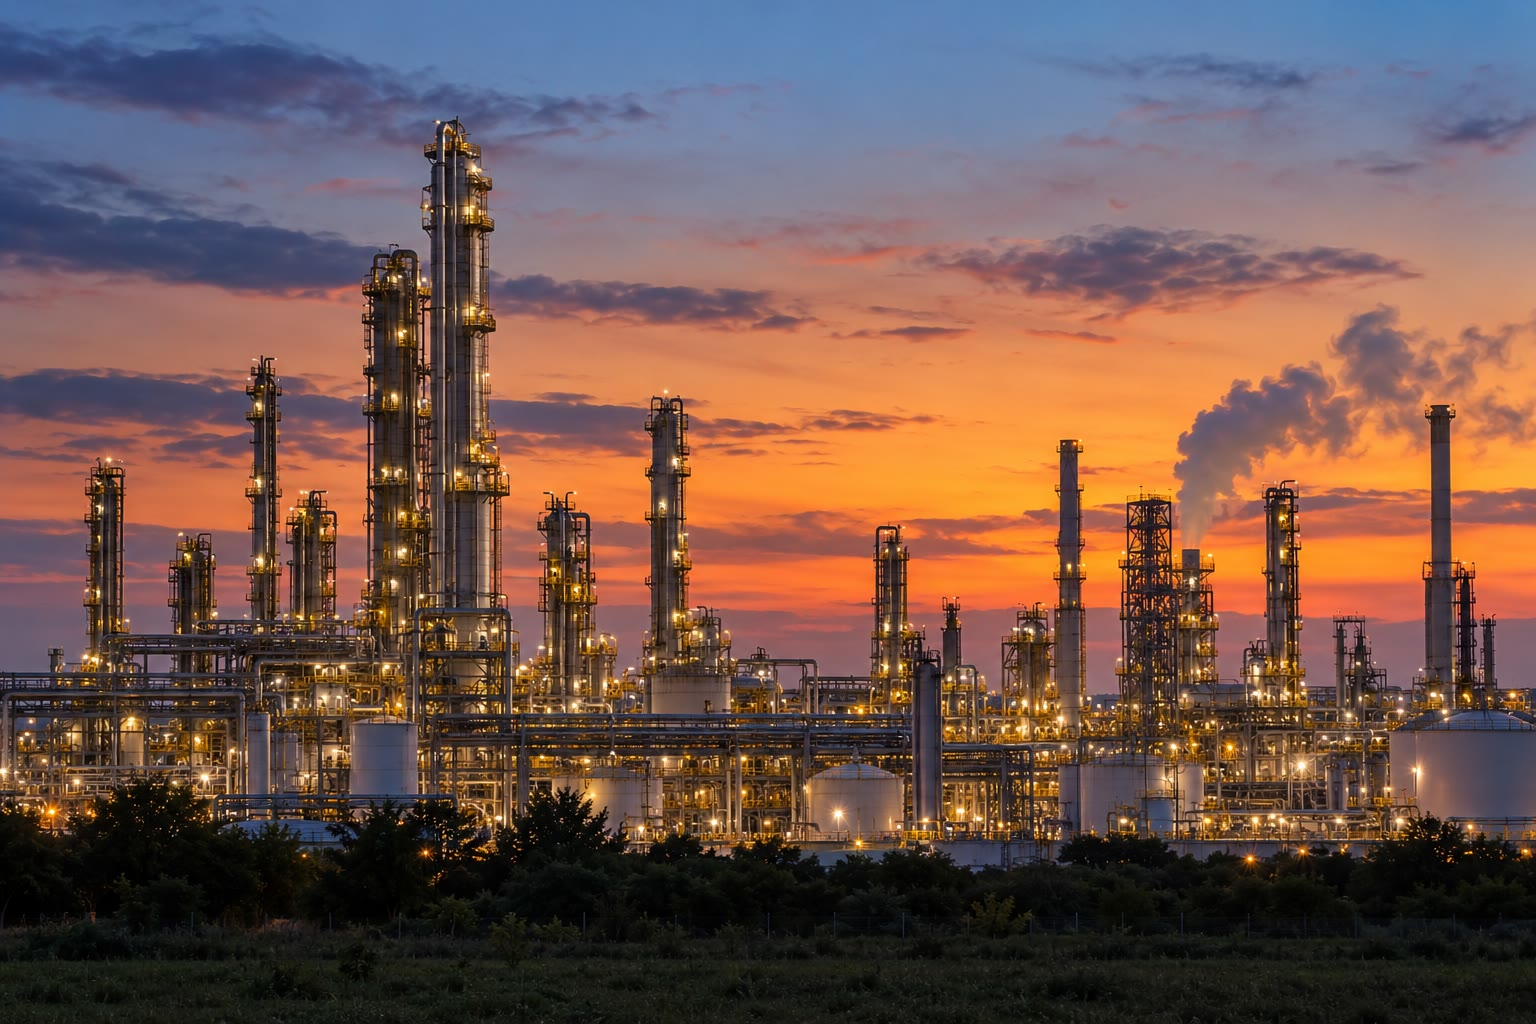
\includegraphics[width=0.6\linewidth]{images/book4/ai/b3-21-chemical-plant.jpg}

{\small 黄昏时分的一座大型化工厂。\omterm{def:b3:homogeneous-catalysis:carbonylation}{羰基化}装置中，催化剂
是溶于反应液中的金属配合物；装置中大部分
物质可分离并循环使用。}
\end{omfigure}

\section{催化氢化}

\begin{method}[读懂催化循环]\label{met:b3:homogeneous-catalysis:read-cycle}
\begin{enumerate}
  \item 对每种物种，数出价电子数，并给出
        金属的氧化态和 $d^n$。
  \item 为每一步命名（配体的失去或加入、氧化加成、
        插入、消除），并检查计数是否按要求变化
        （氧化加成：氧化态和电子计数各增加 $+2$）。
  \item 找出休止态（即积累的物种）以及
        决速步；速率方程由各物种之间的
        预平衡推出。
\end{enumerate}
\end{method}

\begin{omfigure}
\begin{tikzpicture}[font=\small, >=Stealth]
  \node (a) at (90:2.3) {\ce{RhCl(PPh3)2} \ (14 价电子，Rh$^{\mathrm I}$)};
  \node (b) at (0:3.0) {\ce{RhClH2(PPh3)2} \ (16 价电子，Rh$^{\mathrm{III}}$)};
  \node (c) at (-90:2.3) {\ce{RhClH2(RCH=CH2)(PPh3)2} \ （18 价电子）};
  \node (d) at (180:3.1) {\ce{RhClH(CH2CH2R)(PPh3)2} \ （16 价电子）};
  \draw[->, thick] (a) to[bend left=22] node[midway, above right, font=\scriptsize] {$+\,\ce{H2}$, 氧化加成} (b);
  \draw[->, thick] (b) to[bend left=22] node[midway, below right, font=\scriptsize] {$+$ 烯烃} (c);
  \draw[->, thick] (c) to[bend left=22] node[midway, below left, font=\scriptsize] {迁移插入} (d);
  \draw[->, thick] (d) to[bend left=22] node[midway, above left, font=\scriptsize, align=right] {还原 \\ 消除：$-$ 烷烃} (a);
  \node[anchor=south] (p) at (90:3.4) {\ce{RhCl(PPh3)3} \ （16, 预催化剂）};
  \draw[<->, black!50] (p) -- (a) node[midway, right, font=\scriptsize] {$\mp\,\ce{PPh3}$};
\end{tikzpicture}

{\small 威尔金森催化剂催化烯烃氢化的简化循环
（括号内为价电子数）。膦配体脱去后露出一个空配位点，
循环依次加氢、结合烯烃，将其插入 Rh--H 键中，并
经还原消除放出烷烃。}
\end{omfigure}

\begin{proposition}[威尔金森体系动力学]\label{prop:b3:homogeneous-catalysis:wilkinson-rate}
若 $\ce{RhClL3} \rightleftharpoons \ce{RhClL2} + \mathrm L$（$K_1$）与 $\ce{RhClL2} + \ce{H2} \rightleftharpoons \ce{RhClH2L2}$（$K_2$）均为快速
平衡，且二氢化物与烯烃的反应（速率常数 $k$）
为决速步，
\[
  v = \frac{kK_1K_2[\mathrm{Rh}]_{\mathrm{tot}}[\ce{H2}][\text{烯烃}]}{[\mathrm L] + K_1 + K_1K_2[\ce{H2}]},
\]
该速率对氢气饱和，并受外加膦配体 L 抑制。
\end{proposition}

\begin{proof}
$[\ce{RhClL2}] = K_1[\ce{RhClL3}]/[\mathrm L]$ 与 $[\ce{RhClH2L2}] = K_2[\ce{H2}][\ce{RhClL2}]$。将 $[\mathrm{Rh}]_{\mathrm{tot}}$ 写为
三种物种之和，解出二氢化物，得 $[\ce{RhClH2L2}] =
K_1K_2[\ce{H2}][\mathrm{Rh}]_{\mathrm{tot}}/([\mathrm L] + K_1 + K_1K_2[\ce{H2}])$；速率为此值的 $k$ 倍，
再乘以烯烃浓度。
\end{proof}

威尔金森催化剂对无位阻烯烃的氢化
远快于取代烯烃，羰基不受影响：这是拥挤金属中心的
选择性。手性二膦配体可把同一化学转变为
不对称氢化（见\cref{ch:b3:asymmetric-synthesis}）。

\section{催化氢化过程中的羰基化过程}

\begin{definition}[氢甲酰化]\label{def:b3:homogeneous-catalysis:hydroformylation}
\emph{氢甲酰化}\index{氢甲酰化}是指在 C=C 双键上加成一个氢原子
和一个甲酰基（CHO），反应物为 $\ce{H2}$ 与 CO，将烯烃转化为比其多一个碳原子的醛。
\emph{正异比}\index{正异比}是
直链醛与支链醛
的比值。
\end{definition}

最早的工艺使用 $\ce{HCo(CO)4}$，温度约为 150 至 \qty{180}{\celsius}，
压强极高。铑与三苯基膦配合时，在 \qty{100}{\celsius} 左右即可工作，
压强也低得多，并给出更高的\omterm{def:b3:homogeneous-catalysis:hydroformylation}{正异比}：体积较大的
膦配体有利于使金属落在末端碳上的插入。
丙烯生成丁醛，丁醛可氢化为丁醇，或转化为
增塑醇。

\begin{definition}[羰基化]\label{def:b3:homogeneous-catalysis:carbonylation}
\emph{羰基化}\index{羰基化}是指通过与一氧化碳反应，将羰基
引入分子中的过程，该过程由金属配合物催化，
并通过 CO 的迁移插入实现。
\end{definition}

甲醇\omterm{def:b3:homogeneous-catalysis:carbonylation}{羰基化}生成乙酸，$\ce{CH3OH + CO -> CH3COOH}$，在
以铑（孟山都法）或铱（Cativa 法）为催化剂，以碘甲烷
为\omterm{def:b3:surfaces-catalysis:catalyst-design}{助催化剂}：碘化氢将甲醇转化为碘甲烷，金属
将 CO 插入甲基中，生成的碘乙酰水解，
并重新释放出碘化氢。

\begin{omfigure}
\begin{tikzpicture}[font=\small, >=Stealth]
  \node (a) at (90:2.1) {$\ce{[M(CO)2I2]-}$ (16)};
  \node (b) at (0:2.9) {$\ce{[CH3M(CO)2I3]-}$ (18)};
  \node (c) at (-90:2.1) {$\ce{[CH3COM(CO)I3]-}$ (16)};
  \node (d) at (180:2.9) {$\ce{[CH3COM(CO)2I3]-}$ (18)};
  \draw[->, thick] (a) to[bend left=22] node[midway, above right, font=\scriptsize, align=left] {$+\,\ce{CH3I}$\\ 氧化加成} (b);
  \draw[->, thick] (b) to[bend left=22] node[midway, below right, font=\scriptsize] {迁移插入} (c);
  \draw[->, thick] (c) to[bend left=22] node[midway, below left, font=\scriptsize] {$+$ CO} (d);
  \draw[->, thick] (d) to[bend left=22] node[midway, above left, font=\scriptsize, align=right] {还原消除 \\ $-\,\ce{CH3COI}$} (a);
  \node[anchor=north, align=center, font=\scriptsize] at (0,-2.55) {$\ce{CH3COI + H2O -> CH3COOH + HI}$, \quad $\ce{CH3OH + HI -> CH3I + H2O}$};
\end{tikzpicture}

{\small 甲醇\omterm{def:b3:homogeneous-catalysis:carbonylation}{羰基化}循环，$\mathrm M = \mathrm{Rh}$（孟山都法）；价
电子计数标于括号内，金属氧化数在顶部为 I，其余处为 III。
以铑为催化剂时，碘甲烷的氧化加成为决速步。以
铱（Cativa 法）时该步快得多，迁移插入较慢，并且
能从 $\ce{[CH3Ir(CO)2I3]-}$ 中移除一个碘离子的\omterm{def:b3:surfaces-catalysis:catalyst-design}{助催化剂}可加速插入。}
\end{omfigure}

\begin{proposition}[铑法的速率方程]\label{prop:b3:homogeneous-catalysis:monsanto-rate}
若碘甲烷对 $\ce{[Rh(CO)2I2]-}$ 的氧化加成为决速步，且
该配合物为静止态，$v = k[\mathrm{Rh}]_{\mathrm{tot}}[\ce{CH3I}]$，对 CO 及
甲醇均为零级。
\end{proposition}

\begin{proof}
速率即慢步的速率 $k[\ce{[Rh(CO)2I2]-}][\ce{CH3I}]$，且几乎全部铑
都处于静止态。CO 仅在慢步之后参与，甲醇仅
用于再生碘甲烷，其稳态浓度由加入反应器的碘化物决定，
而非由甲醇决定。
\end{proof}

出于实际原因，新建装置多采用铱而非铑：其配合物
在较低水浓度下仍留在溶液中，从而节省干燥产物的能耗，
且副产物更少。两者的主要副反应是
水煤气变换反应 $\ce{CO + H2O -> CO2 + H2}$，由同一金属催化，会消耗
一氧化碳。

\section{烯烃复分解}

\begin{definition}[烯烃复分解]\label{def:b3:homogeneous-catalysis:metathesis}
\emph{烯烃复分解}\index{烯烃复分解}是指两个烯烃的
亚烷基部分相互交换的过程，$\mathrm{RCH{=}CHR + R'CH{=}CHR' \rightleftharpoons 2\,RCH{=}CHR'}$，由
金属\omterm{def:b3:organometallic-bonding:carbene}{卡宾配合物}催化，经由\emph{金属环丁烷}\index{金属环丁烷}，
即由金属与三个碳构成的四元环。其合成形式包括
\emph{关环复分解}\index{关环复分解}（RCM），它将同一分子的
两个烯端连接成环，并失去乙烯；
\emph{开环复分解聚合}\index{开环复分解聚合}
（ROMP）适用于张力环状烯烃，以及\emph{交叉
复分解}\index{交叉复分解}，指两种不同烯烃之间的反应。
\end{definition}

\begin{definition}[肖万机理]\label{def:b3:homogeneous-catalysis:chauvin}
复分解的\emph{肖万机理}\index{肖万机理}是指
以 $[2+2]$ 环加成的方式，烯烃与金属\omterm{def:b3:organometallic-bonding:carbene}{卡宾} $\mathrm{[M]{=}CHR}$ 结合，生成
\omterm{def:b3:homogeneous-catalysis:metathesis}{金属环丁烷}，随后沿另一方向进行环逆反应，
释放出新烯烃和新\omterm{def:b3:organometallic-bonding:carbene}{卡宾}。
\end{definition}

\begin{omfigure}
\setchemfig{atom sep=2.1em}
\schemestart
\chemfig{M=[:0]CHR}
\+
\chemfig{R'HC=[:0]CHR'}
\arrow{<=>}
\chemfig{M?-[:0]CHR-[:-90]CHR'-[:180]CHR'?}
\arrow{<=>}
\chemfig{M=[:0]CHR'}
\+
\chemfig{RHC=[:0]CHR'}
\schemestop
\par\vspace{10pt}

{\small \omterm{def:b3:homogeneous-catalysis:chauvin}{肖万机理}：金属\omterm{def:b3:organometallic-bonding:carbene}{卡宾}与烯烃结合为
\omterm{def:b3:homogeneous-catalysis:metathesis}{金属环丁烷}，再沿另一方向开环，生成新\omterm{def:b3:organometallic-bonding:carbene}{卡宾}和
新烯烃。每一步均为可逆反应：除非有
产物离开，复分解会达到平衡。}
\end{omfigure}

\begin{proposition}[推动关环复分解]\label{prop:b3:homogeneous-catalysis:metathesis-equilibrium}
对于成环反应 $\text{二烯} \rightleftharpoons \text{环烯} + \ce{C2H4}$，将乙烯从
溶液中移去，可使反应进行到底；该反应
受释放一个气体分子所带来的熵增推动。
\end{proposition}

\begin{proof}
平衡时 $K = [\text{环}][\ce{C2H4}]/[\text{二烯}]$：若通过吹扫或
抽真空使 $[\ce{C2H4}]$ 维持在较低水平，则 $[\text{环}]/[\text{二烯}] = K/[\ce{C2H4}]$ 无限增大。反应中分子数
增加一个，而所形成与断裂的键（各为一个 C=C）
性质相当：对于无张力环，$\Delta_rH^\circ \approx 0$，且 $\Delta_rS^\circ > 0$，因此 $K$ 有利。
\end{proof}

张力环（如降冰片烯）的\omterm{def:b3:homogeneous-catalysis:metathesis}{开环复分解聚合}（ROMP）则
出于相反的原因反向进行：环张力的释放足以抵偿平动熵的损失。
罗伯特·格拉布斯的钌\omterm{def:b3:organometallic-bonding:carbene}{卡宾}能耐受水、空气及大多数
官能团；理查德·施罗克的钼、钨亚烷基配合物活性更高，
并可实现对映选择性。

\section{钯催化交叉偶联}

\begin{definition}[交叉偶联反应]\label{def:b3:homogeneous-catalysis:cross-coupling}
\emph{交叉偶联反应}\index{交叉偶联反应}是指将两个
不同的碳片段连接起来，分别为有机卤化物与有机金属试剂或
烯烃，通常在金属催化剂（多为钯）上进行。在\emph{赫克
反应}\index{赫克反应}中，芳基或乙烯基卤化物与烯烃偶联，
生成取代烯烃；在\emph{铃木–宫浦
偶联}\index{铃木–宫浦偶联}中，它与有机硼
化合物在碱存在下偶联。
\end{definition}

\begin{omfigure}
\begin{tikzpicture}[font=\small, >=Stealth]
  \node (a) at (90:2.0) {$\mathrm{Pd^0L_2}$};
  \node (b) at (0:2.6) {$\mathrm{ArPd^{II}XL_2}$};
  \node (c) at (-90:2.0) {$\mathrm{ArPd^{II}Ar'L_2}$};
  \draw[->, thick] (a) to[bend left=25] node[midway, above right, font=\scriptsize, align=left] {$+\,$ArX\\ 氧化加成} (b);
  \draw[->, thick] (b) to[bend left=25] node[midway, below right, font=\scriptsize, align=left] {$+\,\mathrm{Ar'B(OH)_2}$, 碱 \\ 转金属化} (c);
  \draw[->, thick] (c) to[bend left=35] node[midway, left, font=\scriptsize, align=right] {还原消除 \\ $-\,$Ar--Ar$'$} (a);
\end{tikzpicture}

{\small 铃木–宫浦循环：钯(0)插入芳基卤化物的 C--X 键，
从经碱活化的硼酸处接受第二个芳基，
并通过还原消除释放联芳基。}
\end{omfigure}

\begin{method}[选择交叉偶联方法]\label{met:b3:homogeneous-catalysis:choose-coupling}
\begin{enumerate}
  \item 切断待构建的 C--C 键，一个组分为卤化物，
        其活性次序为：碘化物 $>$ 溴化物 $>$ 三氟甲磺酸酯 $>$ 氯化物；另一个组分则为
        硼酸（\omterm{def:b3:homogeneous-catalysis:cross-coupling}{铃木–宫浦偶联}）、烯烃（\omterm{def:b3:homogeneous-catalysis:cross-coupling}{赫克反应}）、有机锌试剂
        （根岸偶联），或末端炔与亚铜离子（园头偶联）。
  \item 优先选用试剂稳定、易得且毒性最小的组分对：
        联芳基宜用硼酸。
  \item 为最困难的步骤选择配体：富电子、体积大的膦或
        \omterm{def:b3:organometallic-bonding:carbene}{氮杂环卡宾}可加速氯化物的氧化加成。
  \item 规划从产物中脱除钯，
        使其残留量降至药物中允许的低水平（使用清除树脂、结晶等方法）。
\end{enumerate}
\end{method}

\section{聚合催化}

\begin{definition}[齐格勒–纳塔催化]\label{def:b3:homogeneous-catalysis:ziegler-natta}
称\emph{齐格勒–纳塔催化剂}\index{齐格勒–纳塔催化剂}可在低压下使烯烃聚合，
它由过渡金属卤化物（多为钛的卤化物）与烷基铝化合物制成。链增长的
\emph{科西–阿尔曼机理}\index{科西–阿尔曼机理}是：烯烃在金属上与增长烷基链呈顺式的
空配位点处配位，随后插入金属–碳键，
使空配位点重新出现。
\emph{单活性中心催化剂}\index{单活性中心催化剂}的所有活性中心
彼此相同，
如分子型\omterm{def:b3:organometallic-bonding:metallocene}{茂金属}催化剂。
\end{definition}

\begin{omfigure}
\begin{tikzpicture}[font=\small, >=Stealth]
  \begin{scope}[every node/.style={inner sep=1pt}]
  % panel 1: chain and vacant site
  \node (m1) at (0,0) {M};
  \node (p1) at (-0.7,0.55) {P};
  \node (v1) at (0.7,0.55) {$\square$};
  \draw (m1) -- (p1);
  % panel 2: alkene bound side-on at the vacant site
  \node (m2) at (3.6,0) {M};
  \node (p2) at (2.9,0.55) {P};
  \node (c2a) at (4.75,1.25) {\ce{CH2}};
  \node (c2b) at (4.75,0.25) {\ce{CH2}};
  \draw (m2) -- (p2);
  \draw[double, double distance=1.6pt] (c2a) -- (c2b);
  \draw[dashed] (m2) -- (4.55,0.75);
  % panel 3: chain longer by two carbons, vacant site moved
  \node (m3) at (7.7,0) {M};
  \node (v3) at (7.0,0.55) {$\square$};
  \node (c3a) at (8.45,0.55) {\ce{CH2}};
  \node (c3b) at (8.45,1.45) {\ce{CH2}};
  \node (p3) at (7.75,1.95) {P};
  \draw (m3) -- (c3a) -- (c3b) -- (p3);
  \end{scope}
  \draw[->, thick] (1.25,0.35) -- (2.55,0.35) node[midway, above, font=\scriptsize] {$+\,\ce{C2H4}$};
  \draw[->, thick] (5.35,0.35) -- (6.3,0.35) node[midway, above, font=\scriptsize] {插入};
\end{tikzpicture}
\par\medskip

{\small \omterm{def:b3:homogeneous-catalysis:ziegler-natta}{科西–阿尔曼机理}（P：增长的聚合物链；$\square$：
空配位点）。烯烃在链旁结合，
并经由四元过渡态插入 M--C 键；比原来长两个碳的链，
现占据烯烃原先的位置，
空配位点随之移动。}
\end{omfigure}

\begin{proposition}[由催化剂对称性得出的立构规整性]\label{prop:b3:homogeneous-catalysis:tacticity-symmetry}
对于\omterm{def:b3:organometallic-bonding:metallocene}{茂金属}催化剂，若每次插入时链都在两个
配位点之间迁移，则 $C_2$ 对称催化剂得到全同立构聚丙烯，
$C_s$ 对称催化剂得到间同立构聚丙烯。
\end{proposition}

\begin{proof}[论证]
插入的丙烯面由\omterm{def:b3:complex-kinetics:enzyme}{活性位点}的手性环境选定。
在 $C_2$ 对称催化剂中，两个位点由 $C_2$ 轴互换，
该操作保持手性（见\cref{ch:b3:point-groups}）：两个位点选择
相同的面，相继的甲基具有相同的构型（全同立构）。
在 $C_s$ 对称催化剂中，两个位点互为镜像：它们选择
相反的面，构型交替出现（间同立构）。若催化剂的位点
是非手性的，如未桥连的 $\ce{Cp2ZrCl2}$ 与甲基铝氧烷体系，则得到
无规立构的聚合物。
\end{proof}

\begin{proposition}[舒尔茨–弗洛里分布]\label{prop:b3:homogeneous-catalysis:schulz-flory}
若\omterm{def:b3:homogeneous-catalysis:ziegler-natta}{单活性中心催化剂}上每条增长链以恒定概率 $p$ 加入一个单体，
否则发生转移（终止），则含 $n$ 个单元的链的数分数为
$x_n = (1 - p)p^{n-1}$，且分散度 $M_w/M_n = 1 + p$，对于长链趋于 2。
\end{proposition}

\begin{proof}
含恰好 $n$ 个单元的链增长了 $n - 1$ 次，终止了一次，
概率为 $p^{n-1}(1 - p)$。于是 $\sum nx_n = 1/(1 - p)$（数均），且质量
分数 $w_n = nx_n(1 - p)$，给出质均 $\sum nw_n = (1 + p)/(1 - p)$。二者
之比为 $1 + p$。
\end{proof}

\begin{omfigure}
\begin{tikzpicture}
\begin{axis}[width=0.7\linewidth, height=5.2cm, xmin=0, xmax=200, ymin=0, ymax=1.05,
  axis lines=left, xlabel={$M$ / \unit{kg.mol^{-1}}}, ylabel={单位分数（已标度）},
  tick label style={font=\small}, label style={font=\small},
  legend style={font=\scriptsize, draw=none, at={(0.98,0.98)}, anchor=north east}, legend cell align=left]
\addplot[omDef, line width=1pt] table[x=M_kg, y=x] {figdata/out/bachelor-3-schulz-flory.dat};
\addplot[omThm, line width=1pt] table[x=M_kg, y expr=\thisrow{w}/0.368] {figdata/out/bachelor-3-schulz-flory.dat};
\draw[black!40, dashed] (axis cs:28.05,0) -- (axis cs:28.05,1);
\node[font=\scriptsize, anchor=west] at (axis cs:30,0.5) {$M_n$};
\legend{数分数, 质量分数（按其最大值标度）}
\end{axis}
\end{tikzpicture}

{\small 由\omterm{def:b3:homogeneous-catalysis:ziegler-natta}{单活性中心催化剂}制得的聚乙烯，其最可几摩尔质量分布
（模型：平均聚合度为 1000）：数分数指数衰减，
质量分数在 $M_n \approx \qty{28}{kg/mol}$ 处达到峰值；$M_w = 2M_n$。
经典的\omterm{def:b3:homogeneous-catalysis:ziegler-natta}{齐格勒–纳塔催化剂}含多种活性中心，
所得分布较宽。}
\end{omfigure}

\begin{inthelab}[铃木–宫浦偶联及其钯]
芳基溴、硼酸（1.2 当量）、碳酸钾以及
十分之几个百分点的钯膦配合物，在
氮气保护下、经除气的甲苯、乙醇和水的混合物中加热回流搅拌。后处理后，
粗联芳基化合物与能结合钯的巯基功能化硅胶搅拌，
过滤并结晶；残留的钯用
等离子体质谱法测定。
\end{inthelab}

\begin{safety}{\ghs[0.62cm]{GHS02}\ghs[0.62cm]{GHS04}\ghs[0.62cm]{GHS06}\ghs[0.62cm]{GHS08}}
% ledger: ghs4:MeI, ghs:CO
碘甲烷：吸入和误食有毒，接触皮肤有害，疑为
致癌物，易挥发，须在通风橱中操作。一氧化碳：极易燃，吸入有毒，
可能损害胎儿，无味；
使用时须配固定式探测器和报警器。
\end{safety}

\begin{history}[齐格勒、纳塔与烯烃复分解]
卡尔·齐格勒于 1953 年发现，氯化钛与烷基铝化合物
可在常压下使乙烯聚合；朱利奥·纳塔于 1954 年发现，此类
催化剂可制得立构规整的聚丙烯；两人共同获得 1963 年
诺贝尔化学奖。伊夫·肖万于 1971 年提出复分解的\omterm{def:b3:homogeneous-catalysis:metathesis}{金属环丁烷}机理；
与罗伯特·格拉布斯、理查德·施罗克一道（二人制得了结构确定的
复分解催化剂），他于 2005 年获得诺贝尔化学奖。
\end{history}

\section{练习}

\begin{exercise}[$\star$]\label{exo:b3:homogeneous-catalysis:1}
求图中威尔金森循环各步骤中铑的价电子计数和
氧化数。
\end{exercise}

\begin{exercise}[$\star$]\label{exo:b3:homogeneous-catalysis:2}
写出丙烯\omterm{def:b3:homogeneous-catalysis:hydroformylation}{氢甲酰化}生成的两种醛的名称，其中哪一种是
直链醛？
\end{exercise}

\begin{exercise}[$\star$]\label{exo:b3:homogeneous-catalysis:3}
二烯丙基丙二酸二乙酯 $\ce{(CH2=CHCH2)2C(CO2Et)2}$ 发生\omterm{def:b3:homogeneous-catalysis:metathesis}{关环复分解}反应。
求产物及其环的大小。
\end{exercise}

\begin{exercise}[$\star$]\label{exo:b3:homogeneous-catalysis:4}
求碘苯与丙烯酸甲酯发生\omterm{def:b3:homogeneous-catalysis:cross-coupling}{赫克反应}的产物，并说明其
构型。
\end{exercise}

\begin{exercise}[$\star\star$]\label{exo:b3:homogeneous-catalysis:5}
以铑法的循环为出发点，推导其速率方程，并解释
为何在甲醇基本转化完全前，其转化程度不影响反应速率。
\end{exercise}

\begin{exercise}[$\star\star$]\label{exo:b3:homogeneous-catalysis:6}
对 4-甲基联苯提出两种\omterm{def:b3:homogeneous-catalysis:cross-coupling}{铃木–宫浦偶联}的切断方式，并选择其中一种。
\end{exercise}

\begin{exercise}[$\star\star$]\label{exo:b3:homogeneous-catalysis:7}
预测分别用 $C_2$ 对称的桥联双（茚基）锆催化剂、
$C_s$ 对称催化剂和无桥联的 $\ce{Cp2ZrCl2}$ 所制聚丙烯的立构规整性。
\end{exercise}

\begin{exercise}[$\star\star$]\label{exo:b3:homogeneous-catalysis:8}
催化剂用量为 \qty{0.10}{mol\%}，某氢化反应在 \qty{2.0}{h} 内转化率达到 98\,\%。
求转化数及平均转化频率。
\end{exercise}

\begin{exercise}[$\star\star$]\label{exo:b3:homogeneous-catalysis:9}
画出由降冰片烯开环复分解制得的聚合物的重复单元，
并解释该反应为何能进行到底。
\end{exercise}

\begin{exercise}[$\star\star\star$]\label{exo:b3:homogeneous-catalysis:10}
某\omterm{def:b3:homogeneous-catalysis:ziegler-natta}{单活性中心催化剂}得到的链满足 $p = 0.9995$。求数均
聚合度和分散度。为何齐格勒–纳塔
聚合物的分布较宽？
\end{exercise}

\begin{exercise}[$\star\star\star$]\label{exo:b3:homogeneous-catalysis:11}
由威尔金森速率方程证明：低压下反应对 $\ce{H2}$ 为一级，
高压下与之无关，并证明加入膦
会减慢反应。
\end{exercise}

\begin{exercise}[$\star\star\star$]\label{exo:b3:homogeneous-catalysis:12}
解释为何体积较大的膦能提高铑催化
\omterm{def:b3:homogeneous-catalysis:hydroformylation}{氢甲酰化}中的\omterm{def:b3:homogeneous-catalysis:hydroformylation}{正异比}，并说明高\omterm{def:b3:homogeneous-catalysis:hydroformylation}{正异比}
对由这些醛制得的增塑剂醇为何重要。
\end{exercise}

\section{问题：从甲醇到醋酸}

\begin{problem}[{周末问题——铱循环中从甲醇到醋酸：
循环的价电子计数与步骤、决速步与助催化剂、一座工厂的
转化频率，以及因水煤气变换
反应而损失的一氧化碳}]
\label{pb:b3:homogeneous-catalysis:1}
% ledger: aw:Ir, aw:C, aw:H, aw:O
某醋酸工厂（数据见本题）每年生产 $\qty{5.0e5}{t}$ 醋酸，
运行 \qty{8000}{h}，反应液体积为 \qty{200}{m^3}，其中
含铱 \qty{5.0}{mmol/L}。对一氧化碳的选择性为 94\,\%，其余部分经
水煤气变换反应转化。

\medskip\noindent\textbf{第一部分——循环。}
\begin{enumerate}
  \item 计算 $\ce{[Ir(CO)2I2]-}$ 的价电子计数，并给出其氧化数。
  \item $\ce{CH3I}$ 发生氧化加成：生成物为何？其价电子计数与氧化数各为多少？
  \item 失去碘离子并加入 CO：生成何种中性配合物？
  \item 迁移插入：生成物为何？其价电子计数是多少？
  \item 加入碘离子，再发生碘化乙酰的还原消除，
        哪种物种被再生？
  \item 写出与水、甲醇共同闭合循环的两步有机反应。
  \item 写出总反应。
\end{enumerate}

\medskip\noindent\textbf{第二部分——动力学。}
\begin{enumerate}[resume]
  \item 以铱为催化剂时，哪一步是决速步，
        这与铑有何不同？
  \item 捕获碘离子的\omterm{def:b3:surfaces-catalysis:catalyst-design}{助催化剂}如何加速循环？
  \item 由此预测碘离子浓度会有怎样的依赖关系？
  \item 为何反应速率与甲醇浓度无关？
\end{enumerate}

\medskip\noindent\textbf{第三部分——工厂。}
\begin{enumerate}[resume]
  \item 计算每年生产的醋酸的物质的量。
  \item 计算每小时生产的醋酸的物质的量。
  \item 计算反应器中铱的物质的量及其质量。
  \item 计算转化频率。
  \item 计算每年的转化数。
  \item 计算以千克每立方米每小时表示的时空产率。
\end{enumerate}

\medskip\noindent\textbf{第四部分——水煤气变换。}
\begin{enumerate}[resume]
  \item 写出水煤气变换反应。
  \item 计算每摩尔醋酸消耗的 CO 的物质的量。
  \item 计算每摩尔醋酸生成的 \ce{CO2} 的物质的量。
  \item 计算每吨醋酸排放的 \ce{CO2} 的质量。
  \item 降低水的浓度运行为何有利？又有何限制？
  \item 水煤气变换还生成了何种其他产物？
        它在反应器中为何是个问题？
  \item 给出结果：铱催化剂的转化频率。
\end{enumerate}
\end{problem}
